\chapter{Исследовательская часть}

\section{Технические характеристики}

Технические характеристики устройства,на котором проводились исследования:

\begin{itemize}
	\item Процессор: AMD Ryzen 7 5800H (16) @ 4.46 GHz;
	\item Оперативная память: 16 Г;
	\item Операционная система: Arch Linux x86\_64.
\end{itemize}

\section{Расчёт размера массива}

Расчёт размера массива по варианту производится по формуле:

\begin{equation}
	\label{variant}
	N = \frac{X}{8} + \begin{cases}
		X \% 1000,  &\text{если $\frac{X}{4} \% 10 == 0$,} \\
		\ (\frac{X}{4} \% 10) * (X \% 10) + (\frac{X}{2} \% 10), &\text{иначе},
	\end{cases}
\end{equation}
где $X = 8117$ – номер задачи в redmine.

Для моего варианта $N = 1085$


\section{Трудоёмкость алгоритмов}
Для полученного размера было проведено исследование количества операций сравнения в телах циклов в зависимости от индекса искомого элемента в массиве. Результаты приведены в виде гистограмм, для линейного поиска рисунок \ref{fig:LScomp}, для бинарного поиска рисунки \ref{fig:BScomp} и \ref{fig:BScompasc}. На последнем рисунке столбцы отсортированы по высоте. На всех графиках индекс -1 означает ситуацию, когда искомого элемента в массиве нет.



\begin{figure}
	\centering
	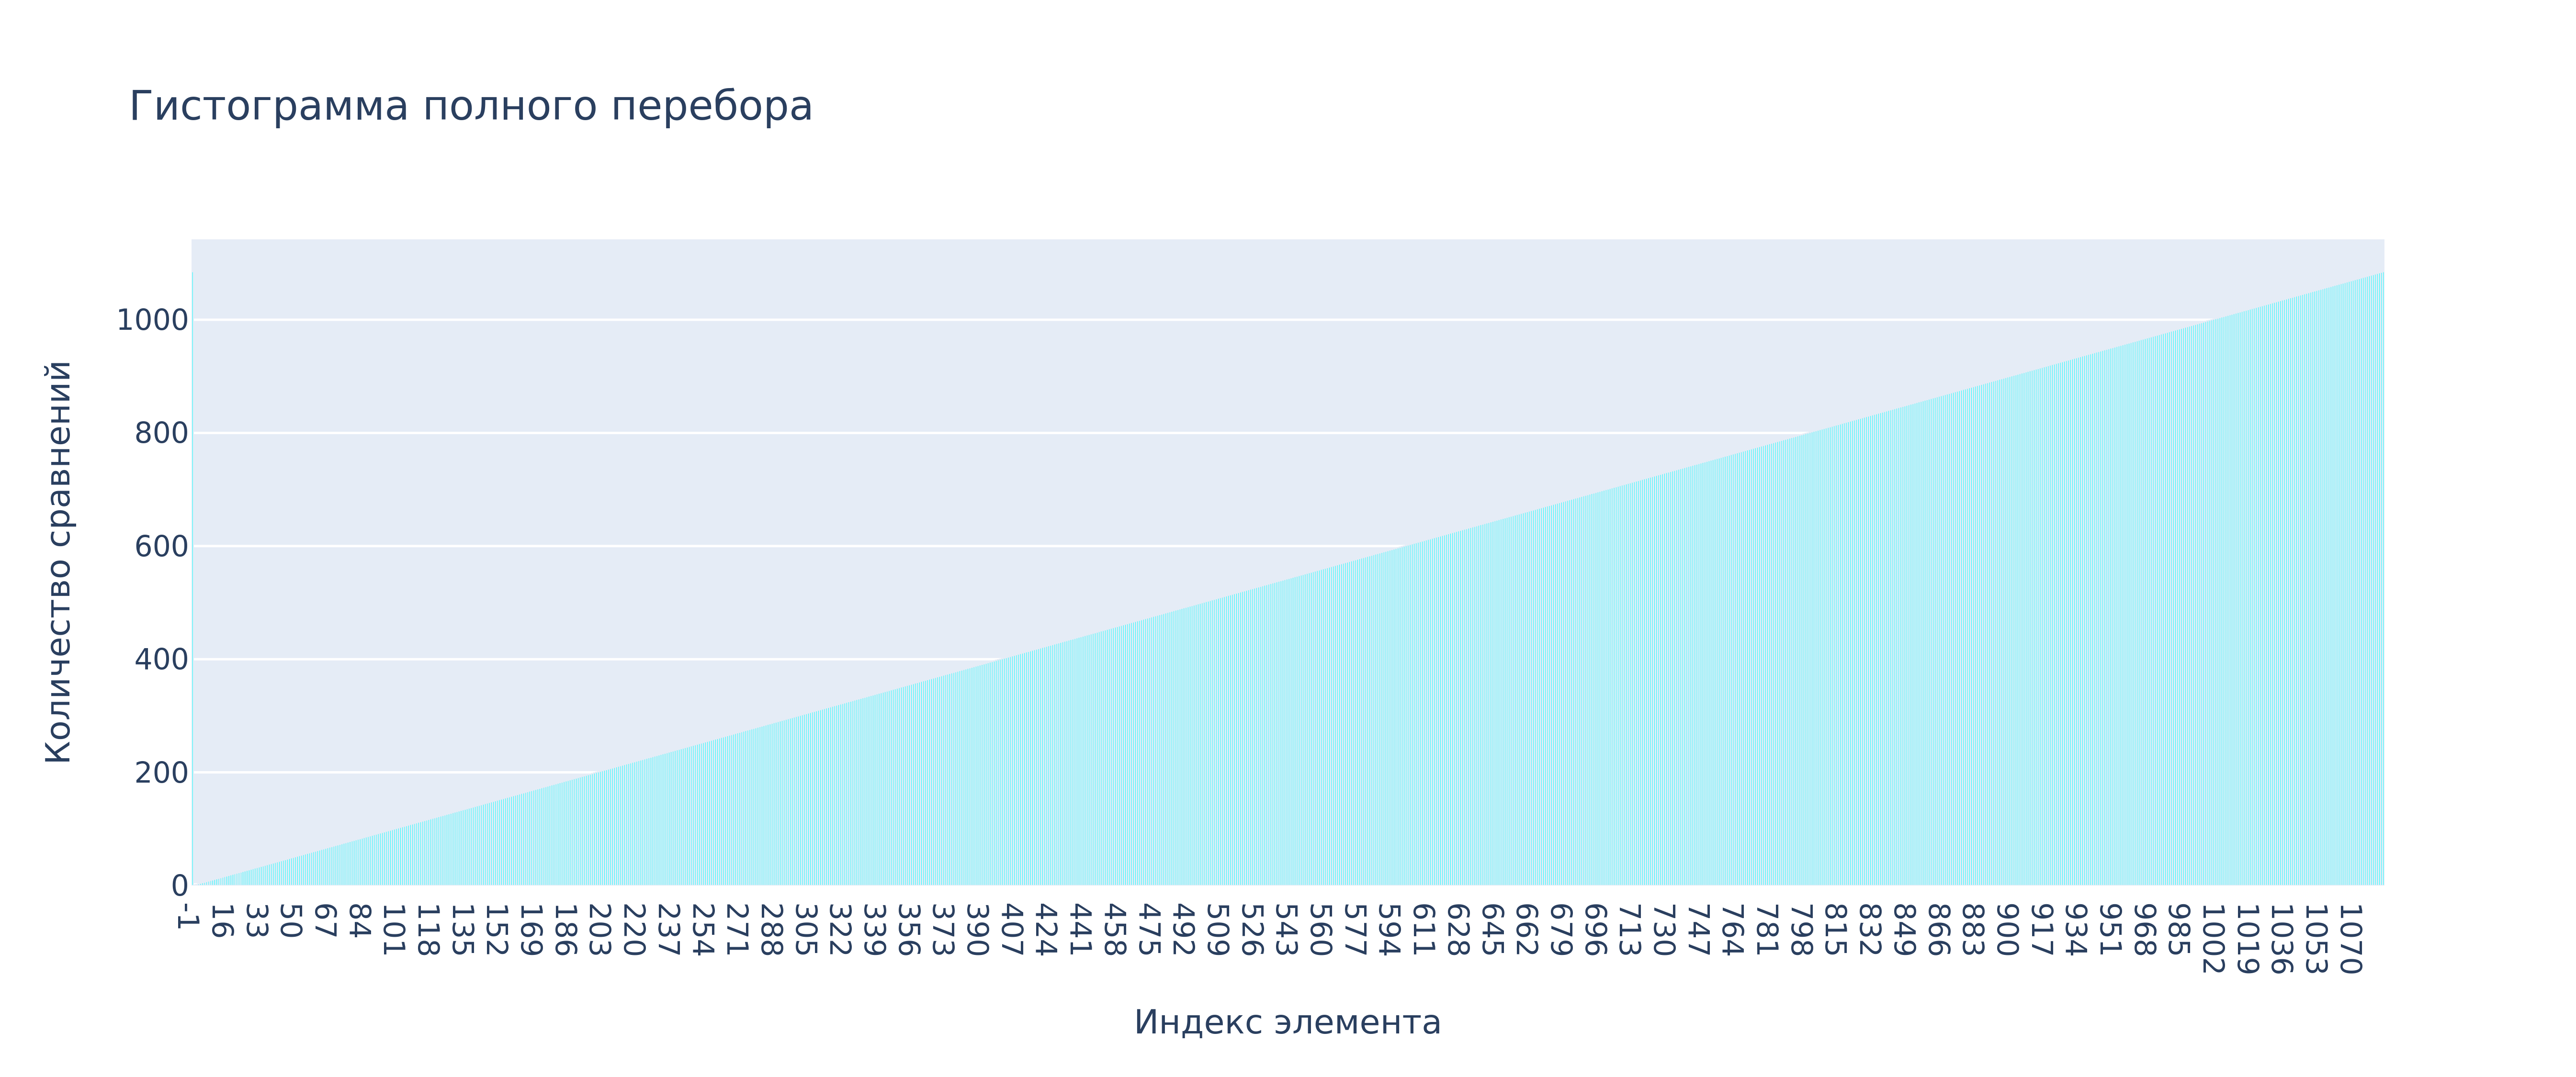
\includegraphics[width=0.9\textwidth]{LScomp}
	\caption{Гистограмма зависимости количества сравнений от индекса элемента в линейном поиске}
	\label{fig:LScomp}
\end{figure}

\begin{figure}
	\centering
	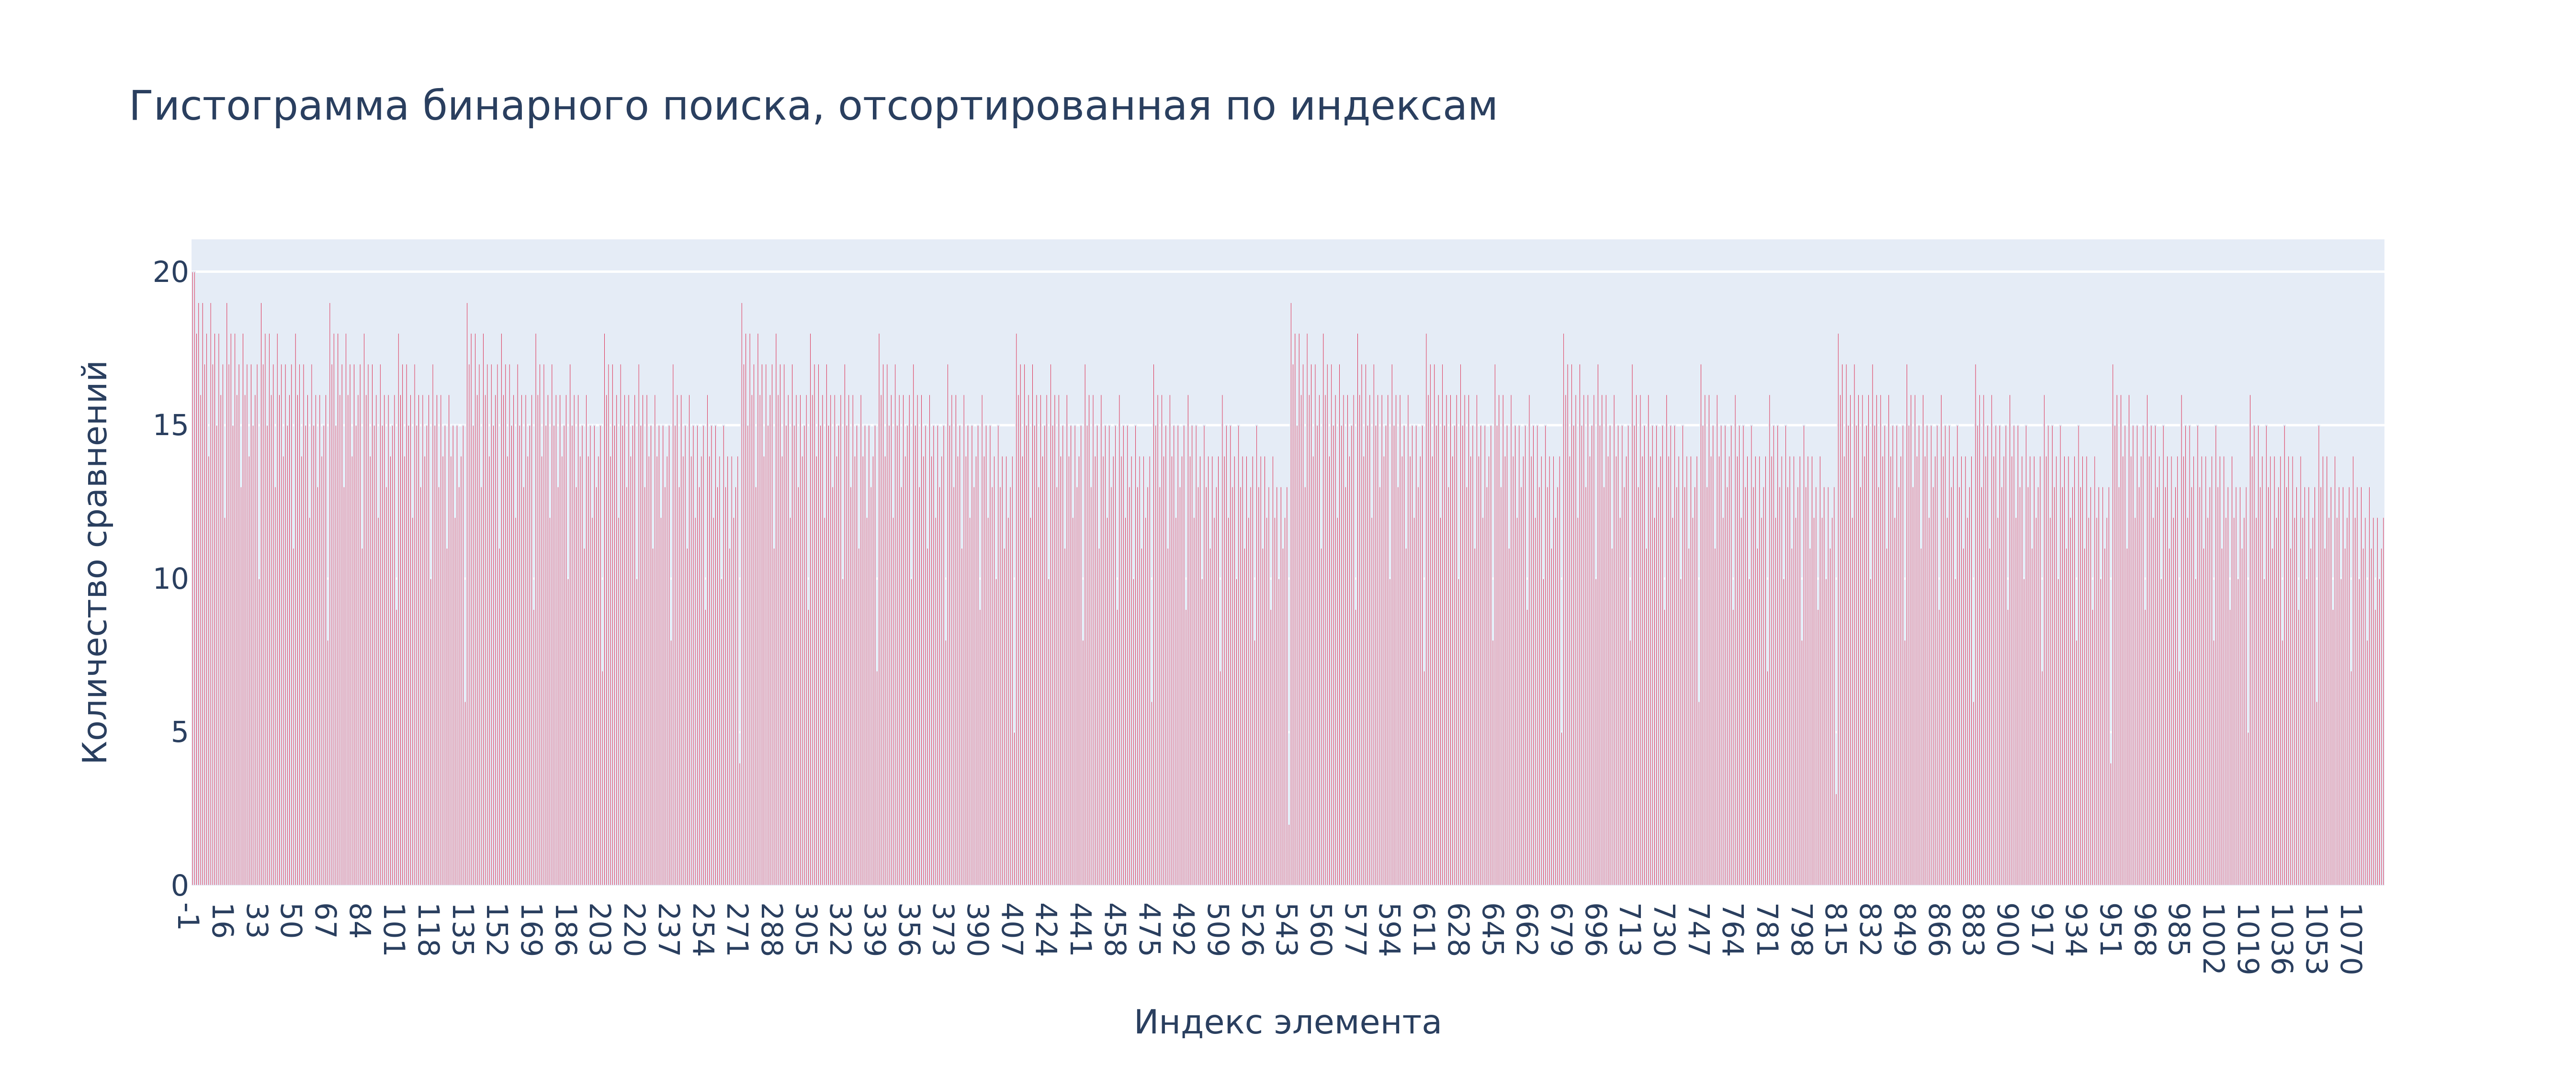
\includegraphics[width=0.9\textwidth]{BScomp}
	\caption{Гистограмма зависимости количества сравнений от индекса элемента в бинарном поиске}
	\label{fig:BScomp}
\end{figure}

\begin{figure}
	\centering
	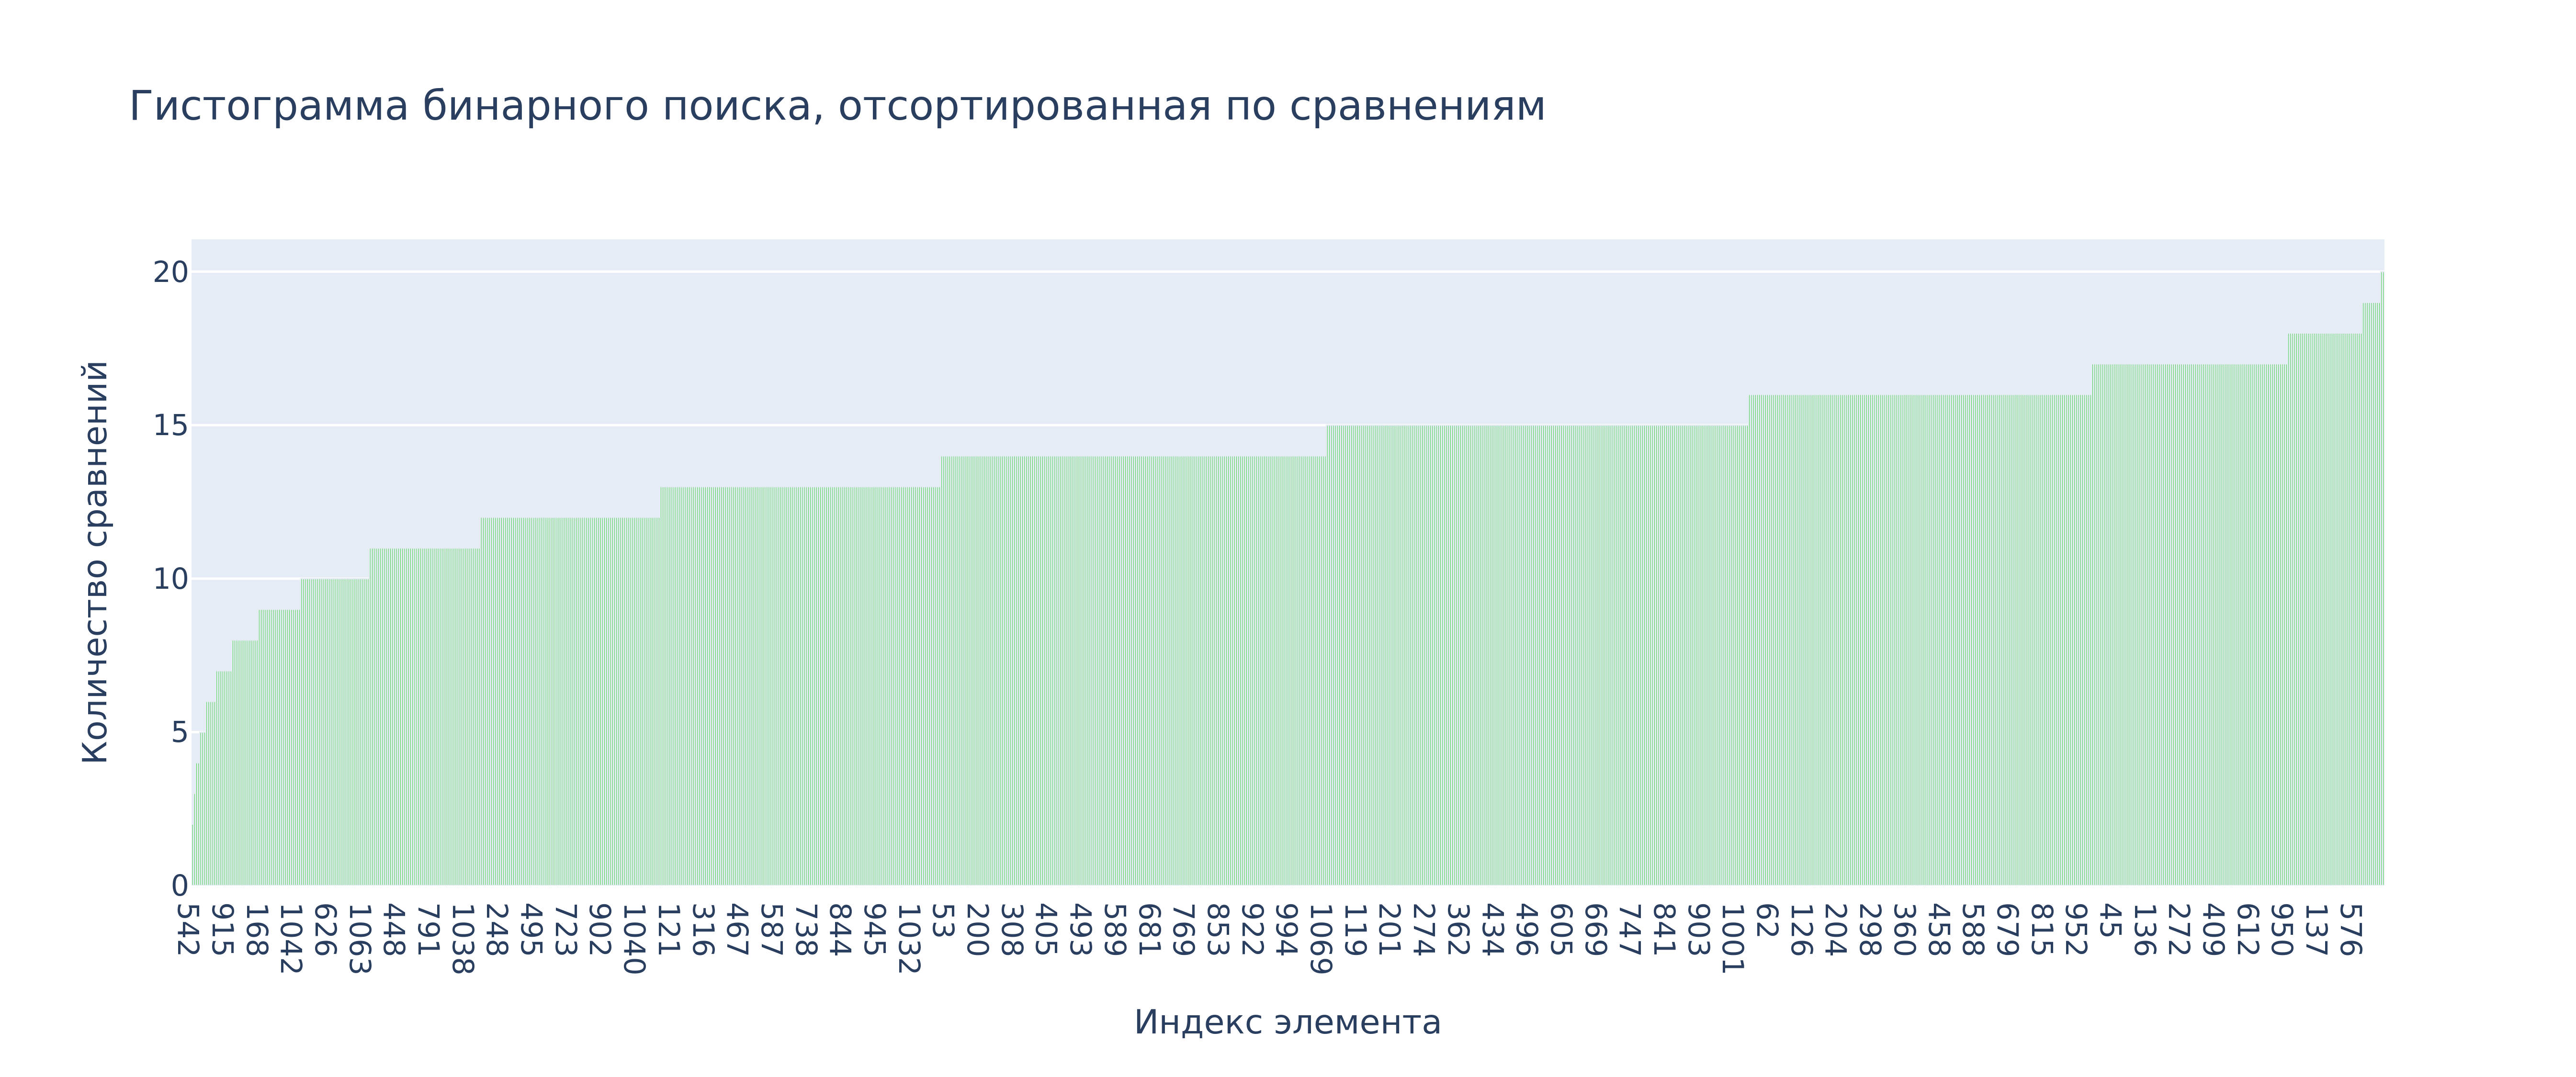
\includegraphics[width=0.9\textwidth]{BScompasc}
	\caption{Гистограмма зависимости количества сравнений от индекса элемента в бинарном поиске, отсортировано по количеству сравнений}
	\label{fig:BScompasc}
\end{figure}

\pagebreak

\section{Вывод}

В данном разделе было проведено исследование трудоёмкости алгоритмов поиска в массиве.

Как видно из рисунков \ref{fig:LScomp}–\ref{fig:BScompasc}, линейный поиск существенно уступает бинарному по количеству операций сравнения. При длине массива 1085 элементов максимальное число сравнений для линейного поиска – 1085, а для бинарного поиска – 20.

Также, как можно отметить на рисунке \ref{fig:BScompasc}, кривая трудоёмкости бинарного поиска имеет форму логарифмической прямой, что подтверждает его логарифмическую сложность O(logN).

\clearpage
